\documentclass[11pt]{beamer}
\usetheme{Madrid}
\usepackage{ctex}
\usepackage{graphicx}

\title{气候变化与环境保护：科学、影响与行动路径}
\author{AI Agent 生成}
\date{\today}

\begin{document}

\maketitle

\tableofcontents
\newpage

\section{引言：为何气候变化是当今最紧迫的全球挑战}

\begin{frame}
\frametitle{引言：为何气候变化是当今最紧迫的全球挑战}
\framesubtitle{本节概览}
\begin{itemize}
    \item \textbf{从环境问题到生存危机}：气候变化已演变为系统性风险，威胁人类文明的根基
    \item \textbf{2023年创纪录数据}：全球平均气温升幅达1.45°C，极端事件年损失超2000亿美元
    \item \textbf{坚如磐石的科学共识}：超过97\%的气候科学家确认人类活动是变暖主因
    \item \textbf{气候与环境的正反馈循环}：生态系统退化削弱碳汇，加速全球变暖
    \item \textbf{本演示文稿的五大支柱}：科学基础、多维影响、应对策略、案例实践与个人行动
\end{itemize}
\end{frame}

\begin{frame}
\frametitle{气候变化的视觉警钟}
\begin{center}

\includegraphics[width=0.7\textwidth]{./3905ed53faf3.jpeg}
\end{center}
\end{frame}

\begin{frame}
\frametitle{图像背后的信息}
\framesubtitle{直观呈现系统性危机的尺度}
\begin{itemize}
    \item 这张图像捕捉了气候变化引发的典型极端事件或生态退化场景——无论是肆虐的野火、消融的冰川，还是被洪水淹没的土地，它们不再是孤立的环境新闻，而是\alert{全球变暖的直接指纹}
    \item 视觉化语言帮助我们将抽象的气温上升数字转化为\alert{可感知的冲击}：基础设施损毁、生物多样性丧失、大量人口流离失所
    \item 正如本节将要展开的，这些现象背后是物理规律、经济代价和人类选择的多重交织，\textbf{每一个画面都在提醒我们行动刻不容缓}
\end{itemize}
\end{frame}

\begin{frame}
\frametitle{从环境议题到系统性生存危机}
\begin{itemize}
    \item \textbf{工业革命以来的“大加速”}：自1750年起，人类对化石能源的依赖使大气中CO$_2$浓度从约280 ppm飙升至目前超过420 ppm，地球系统的运行轨迹被彻底改写
    \item \textbf{风险性质的蜕变}：早期讨论多局限于空气污染或局部生态破坏，而今气候变化已通过\alert{粮食减产、水资源短缺、海平面上升、大规模移民}等渠道，传导至金融稳定、国家安全和公共卫生领域
    \item \textbf{不可逆的临界点逼近}：格陵兰冰盖崩塌、亚马孙雨林荒漠化、大西洋经向翻转环流停摆等\textbf{气候临界点}一旦触发，将引发多米诺骨牌效应，人类将丧失控制力
    \item \textbf{代际正义的拷问}：当今一代的排放正在剥夺后代的基本生存条件，这使得气候变化成为\alert{最深刻的伦理挑战之一}
\end{itemize}
\end{frame}

\begin{frame}
\frametitle{2023年：有记录以来最热的一年}
\framesubtitle{世界气象组织（WMO）关键数据}
\begin{itemize}
    \item \textbf{全球平均气温}：比1850–1900年工业革命前基线高出约1.45°C，刷新历史极值，是自125000年前末次间冰期以来从未有过的高温水平
    \item \textbf{极端事件的代价清单}：全年由气候灾害引发的直接经济损失超过2000亿美元——加拿大野火烧毁近1850万公顷森林，利比亚飓风“丹尼尔”导致超过11000人丧生，南欧热浪使农业收成锐减
    \item \textbf{复合灾害常态化}：同一年份、同一区域可能先后遭遇\alert{极端高温、干旱、暴雨和野火}的多重打击，削弱了社会的恢复力，保险赔付连年创下新高
    \item \textbf{温度只是起点}：比温度本身更可怕的是其引发的\textbf{级联效应}——冰川加速消融威胁淡水供应，海洋热浪摧毁珊瑚礁渔业，冻土融化释放更多温室气体
\end{itemize}
\end{frame}

\begin{frame}
\frametitle{科学共识：人类活动是毋庸置疑的主因}
\framesubtitle{IPCC第六次评估报告的核心结论}
\begin{itemize}
    \item \textbf{97\%以上的共识}：对超过11万篇气候科学论文的分析显示，\alert{97\%以上的学者}认同当今变暖主要由人类活动驱动，化石燃料燃烧和土地利用变化是两大元凶
    \item \textbf{检测与归因的坚实链条}：通过比对仅自然强迫（火山、太阳）和自然+人为强迫的模型模拟，科学家确认\textbf{自1850年以来观测到的约1.1°C升温中，人类活动贡献了几乎全部}
    \item \textbf{温室气体的锁定效应}：二氧化碳的寿命长达数百年，即便立刻停止所有排放，已积存在大气中的温室气体仍将使温度持续上升数十年，这要求我们必须同时推进\alert{深度减排}和\alert{碳移除}
    \item \textbf{不确定性不是拖延的理由}：虽然对云反馈等细节仍有研究空间，但整体结论在统计上已达到“金色标准”，科学上的确定性足以要求紧急行动
\end{itemize}
\end{frame}

\begin{frame}
\frametitle{气候与环境的致命耦合：加速变暖的正反馈}
\framesubtitle{当生态系统从“盟友”变成“加害者”}
\begin{itemize}
    \item \textbf{碳汇退化的现实}：森林、湿地、冻土和海洋吸收了人类排放约56\%的二氧化碳，然而毁林、排水和海洋酸化正使这些自然“海绵”逐渐饱和甚至逆转——\alert{亚马孙部分区域已从碳汇变为碳源}
    \item \textbf{冻土-甲烷定时炸弹}：北极永久冻土层中封存着约1.7万亿吨碳，一旦解冻，微生物分解将释放大量的甲烷和二氧化碳，形成\textbf{自持式的变暖循环}，人类减排努力将被部分抵消
    \item \textbf{野火-碳排放的恶性循环}：高温、干旱导致火灾季延长，野火燃烧又会将数亿吨碳抛入大气并摧毁植被，进一步削弱陆地碳汇能力，2023年加拿大野火的排放量已超过该国全年人为排放的三倍
    \item \textbf{保护自然就是保护气候}：恢复泥炭地、再造林和可持续土地管理不仅是环境议题，更是\alert{最具成本效益的气候解决方案之一}，二者必须协同推进
\end{itemize}
\end{frame}

\begin{frame}
\frametitle{本演示文稿的知识地图}
\framesubtitle{从科学认知走向可操作行动}
\begin{itemize}
    \item \textbf{第一层面：科学基础}——厘清温室效应原理、气候系统运行机制以及未来情景预估，为后续讨论铺设事实基底
    \item \textbf{第二层面：多维影响}——评估气候变化对自然生态系统、社会经济体系、人类健康和地缘安全的深远冲击，揭示风险传导路径
    \item \textbf{第三层面：应对策略}——解析减排（减缓）与适应两大战略，介绍关键技术、政策工具和国际治理框架，如碳定价、可再生能源部署
    \item \textbf{第四层面：案例实践}——展示全球各地的成功探索：从北欧碳中和先锋到非洲“绿长城”生态修复工程，提炼可复制的经验
    \item \textbf{第五层面：个人行动}——打破“个人无足轻重”的迷思，提供碳足迹缩减指南、公民参与渠道和生活方式转型的具体方案，强调\alert{集体行动乘以70亿}的变革力量
\end{itemize}
\end{frame}

\section{气候变化的科学基础：从温室效应到极端天气}

\begin{frame}
\frametitle{气候变化的科学基础：本节概览}
\begin{itemize}
    \item \textbf{温室效应的物理本质}：从自然现象到人类增强
    \item \textbf{关键温室气体}：二氧化碳与甲烷的浓度跃升
    \item \textbf{全球增温格局}：不均衡升温与北极放大效应
    \item \textbf{极端天气的物理机制}：水汽、热浪与热带气旋
\end{itemize}
\end{frame}

\begin{frame}
\frametitle{温室效应：地球的“保温被”}
\begin{itemize}
    \item \textbf{温室效应}是地球大气层中的水汽（H$_2$O）、二氧化碳（CO$_2$）、甲烷（CH$_4$）、氧化亚氮（N$_2$O）等气体吸收地表发射的长波红外辐射，并将其部分能量重新辐射回地面的自然物理过程。没有这个效应，地球表面平均温度将降至约-18°C，而非现在的约15°C。
    
    \item 然而，自工业革命以来，人类活动——尤其是化石燃料燃烧、大规模工业生产和土地利用变化——导致大气中温室气体浓度急剧上升，\alert{人为增强了原本处于精巧平衡的自然温室效应}，造成地球气候系统能量收支失衡，即“辐射强迫”不断增强。
    
    \item 在所有人为温室气体中，\textbf{二氧化碳}因其排放量巨大、大气寿命长达数百年，贡献了约三分之二的辐射强迫增量；而\textbf{甲烷}尽管寿命较短（约12年），但其分子吸收红外辐射的能力极强，在短期内具有远超二氧化碳的增温潜力，这两种气体共同构成了人为气候变暖的核心驱动力。
\end{itemize}
\end{frame}

\begin{frame}
\frametitle{温室效应机制示意图}
\begin{center}
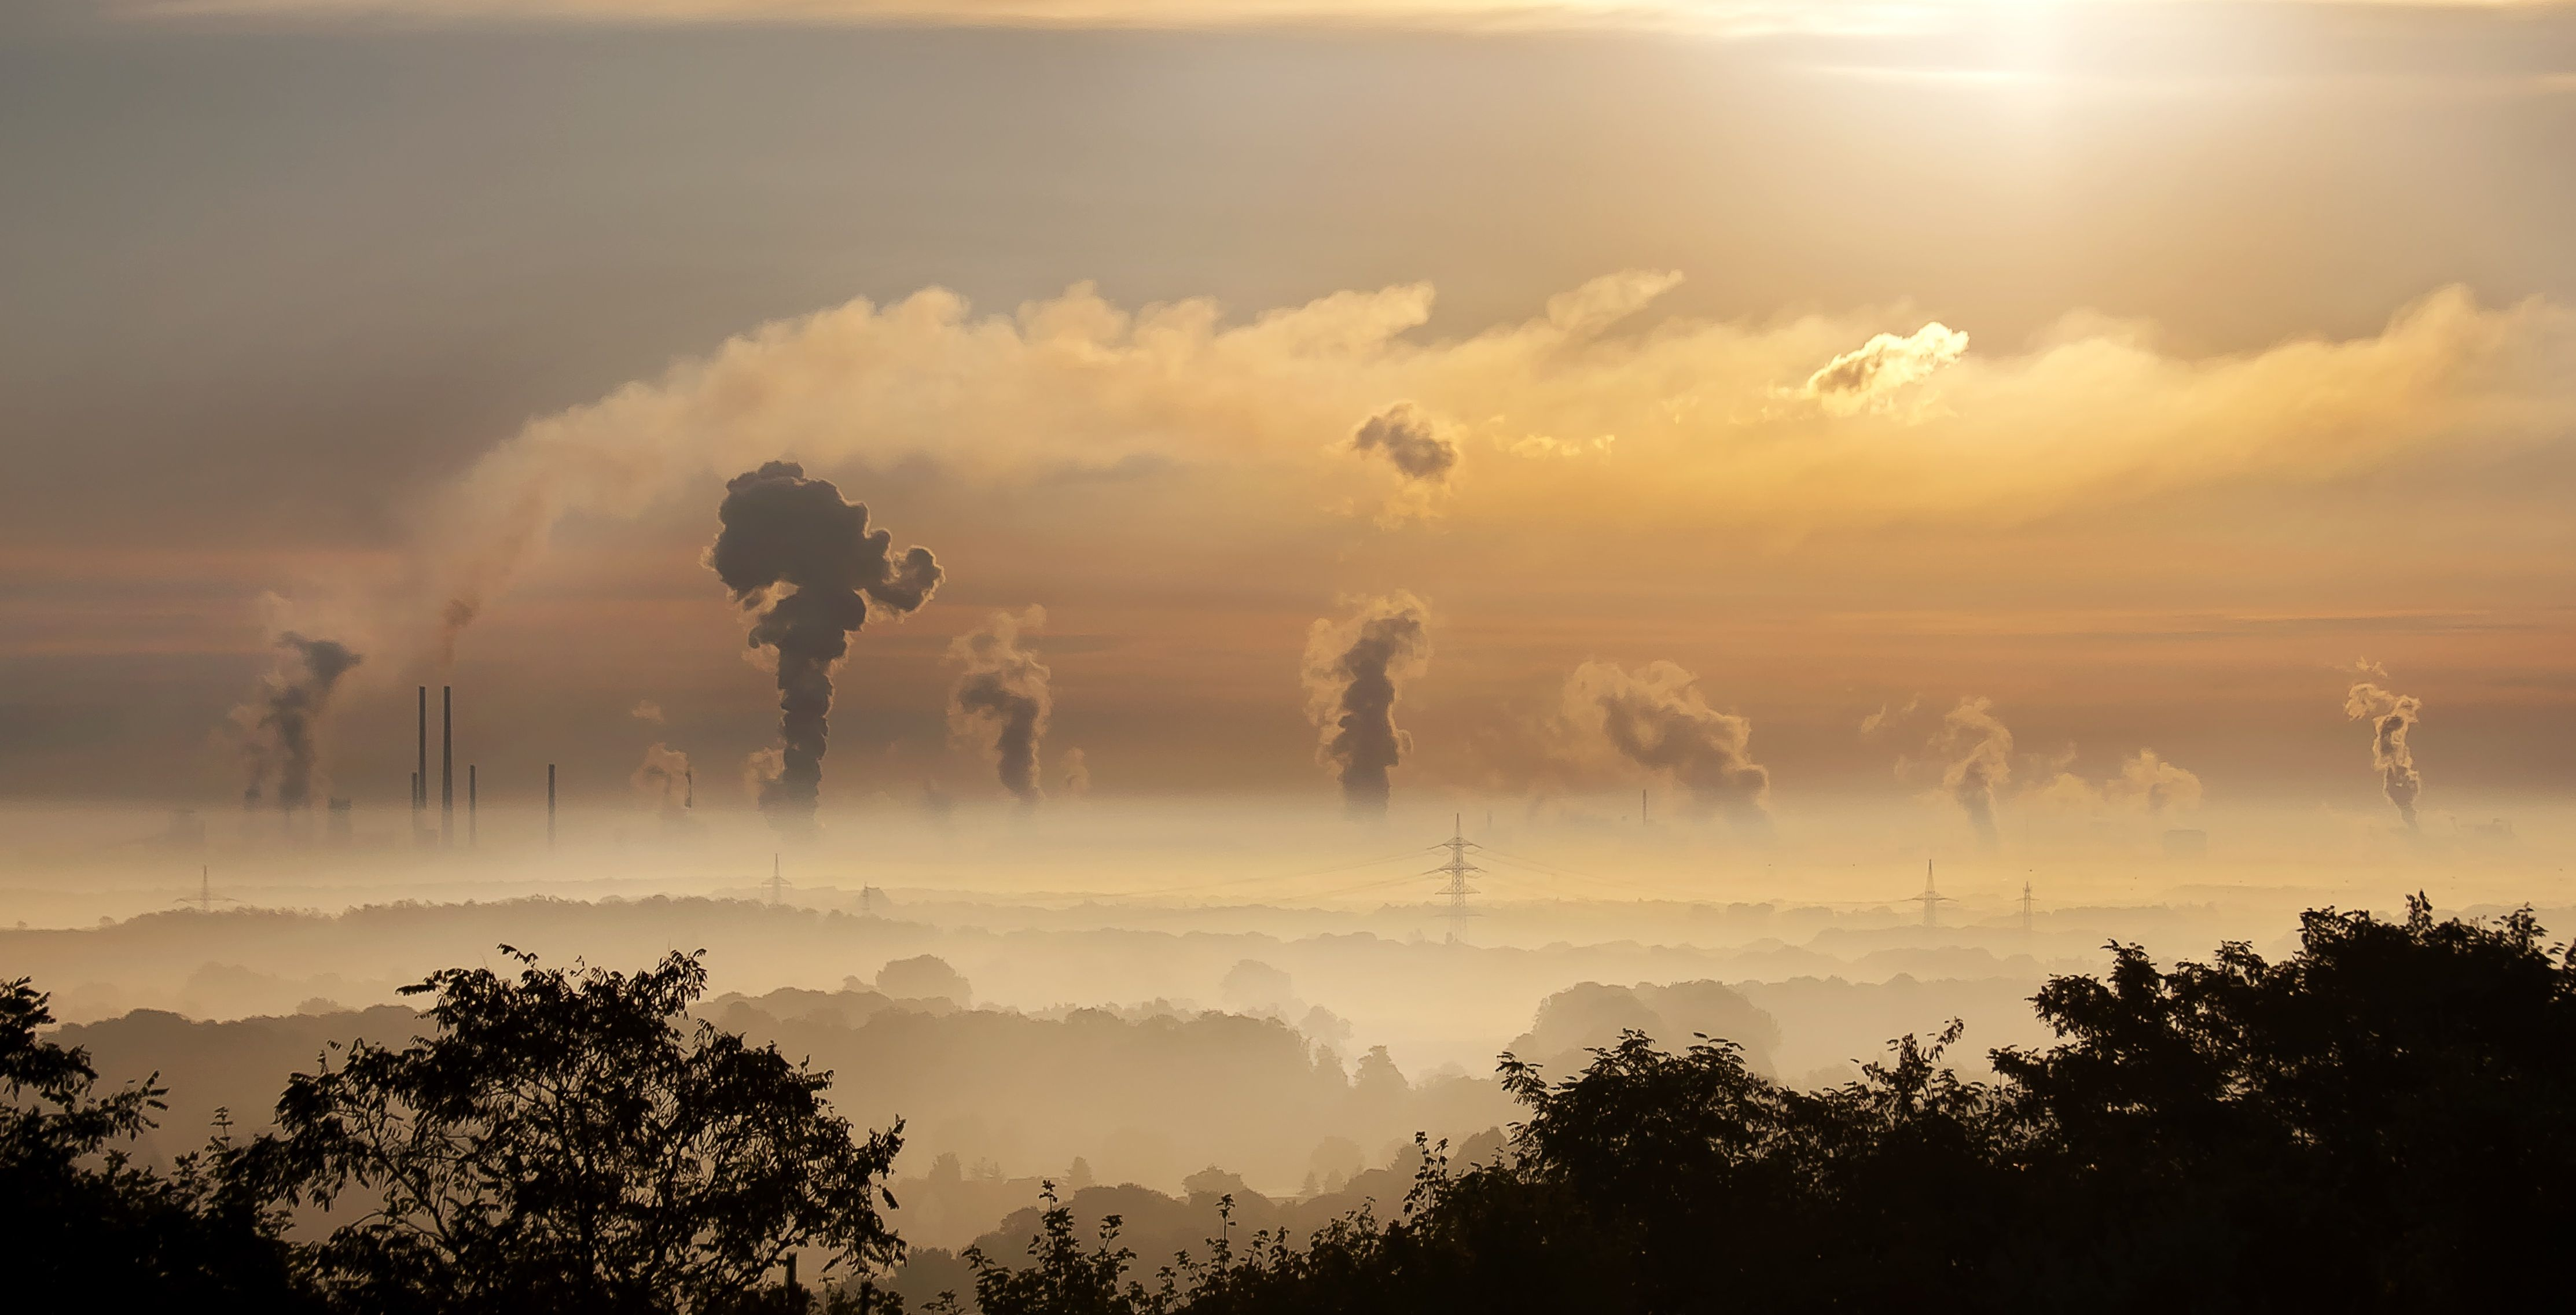
\includegraphics[width=0.7\textwidth]{./5804d64d5e17.jpeg}
\end{center}
\end{frame}

\begin{frame}
\frametitle{图片解读：大气辐射平衡的核心逻辑}
\begin{itemize}
    \item 本图直观展示了地球-大气系统的辐射平衡机制：入射的太阳短波辐射（黄色箭头）一部分被云层和地表反射，另一部分被地表吸收并转化为长波红外辐射向外太空散逸，而大气中的温室气体分子吸收并重新辐射这些长波辐射，形成天然的“保温”效果。
    
    \item 图中红色箭头所指示的\alert{“反向辐射”}正是温室效应的核心——它将本应逃逸到太空的能量截留在对流层内，维持地球适合生命存在的温度。然而，当温室气体浓度持续增加，这份“保温被”就变得越来越厚，打破原有的能量平衡，这正是当下全球变暖最根本的物理学成因。
\end{itemize}
\end{frame}

\begin{frame}
\frametitle{二氧化碳：突破百万年尺度的浓度纪录}
\begin{itemize}
    \item 通过对南极和格陵兰冰芯中封存远古气泡的精确分析，科学家重建了过去80万年间大气二氧化碳浓度的变化历史。在整个冰期-间冰期旋回中，CO$_2$浓度在约170ppm到300ppm之间波动，而工业革命前的一万年间，它稳定在约\textbf{278--280ppm}的狭窄范围内，构成了全新世人类文明发展的稳定气候背景。
    
    \item 位于夏威夷莫纳罗亚火山顶的\alert{莫纳罗亚观测站}自1958年起由查尔斯·基林开始进行大气CO$_2$的连续精密测量，产出了被誉为气候科学“基石”的“基林曲线”。这条曲线不仅揭示了CO$_2$浓度的季节“呼吸”振荡，更记录了一条令人警醒的单调上升轨迹。
    
    \item 截止2023年，莫纳罗亚观测站的年均CO$_2$浓度已突破\alert{约420ppm}，较工业革命前增幅超过50\%。420ppm这个数字在地球近代史上是空前的——上一次大气CO$_2$浓度达到类似水平，可能需要追溯到300万至500万年前的上新世中期，那时全球海平面比现在高出约10至20米。
\end{itemize}
\end{frame}

\begin{frame}
\frametitle{甲烷：短期增温潜力巨大的隐形推手}
\begin{itemize}
    \item 甲烷分子在红外波段拥有比二氧化碳密集得多的吸收谱线，使其单位质量的增温效率极为惊人。在政府间气候变化专门委员会（IPCC）惯用的比较框架中，\alert{甲烷的20年全球增温潜势（GWP$_{20}$）是二氧化碳的84倍}，即在20年时间尺度上，排放一吨甲烷带来的累积辐射强迫相当于排放84吨二氧化碳。
    
    \item 大气甲烷浓度已从工业化前约\alert{722ppb（十亿分之一）}飙升至2022年的约\alert{1911ppb}，增幅超过160\%，而且近年出现了令人困惑的加速增长趋势。同位素指纹分析表明，近期增量主要来自生物源排放，而非化石源。
    
    \item 主要人为排放源包括：\textbf{反刍动物畜牧业}——牛羊等动物的肠道发酵过程；\textbf{水稻种植}——淹水厌氧环境促使产甲烷菌活跃分解有机质；以及\textbf{油气系统泄漏}——从开采、运输到加工过程中的逸散排放。湿地自然排放则在气候变暖背景下存在正反馈风险。
\end{itemize}
\end{frame}

\begin{frame}
\frametitle{全球平均增温：1.1°C背后的加速现实}
\begin{itemize}
    \item 根据美国宇航局戈达德空间研究所和英国哈德莱中心等机构汇编的全球地表气温数据集，自1880年有可靠仪器记录以来，全球平均表面温度已经上升了约\alert{1.1°C}。这一升温幅度在全球广袤海洋的质量惯性下显得尤为巨大。
    
    \item 更值得警惕的是升温速度的剧烈变化。将整个约140年的记录分段审视：1880年至1975年的近一个世纪内，增温速率相对平缓，且存在年代际自然波动；但自\alert{1975年开始}，全球变暖进入了明显的“快车道”，增温速率达到约\alert{每十年0.18°C}，相当于早期速率的数倍。
    
    \item 这一加速拐点与二战后全球经济腾飞、化石能源消费呈指数级增长的“大加速”时期精确吻合。最近的十年（2014-2023年）已是仪器记录中最温暖的十年，2023年更是以显著优势成为有记录以来最热的一年，全球均温较工业化前基线高出约1.45°C，逼近《巴黎协定》的1.5°C警戒线。
\end{itemize}
\end{frame}

\begin{frame}
\frametitle{北极放大效应：暖化不均的典型案例}
\begin{itemize}
    \item 全球变暖并非均匀作用于地球每个角落，其空间分布极度不均衡。其中最显著的现象是\alert{“北极放大效应”}——北极地区的增温速度达到了全球平均水平的\alert{3至4倍}，在西伯利亚沿岸局部区域甚至更高。这使得北极成为了全球气候变化的“响铃区”。
    
    \item 驱动这一效应的物理学机制是多重的：最核心的是\textbf{海冰-反照率正反馈}——随着反射阳光的白色海冰融化，裸露的深色开阔海水吸收了远多于此前被反射回太空的太阳辐射能，导致局地剧烈增温并使更多海冰融化，形成自我强化的反馈循环。
    
    \item 后果已经触目惊心：北极夏季海冰范围以每十年约13\%的速度缩减，格陵兰冰盖正经历千年未有的质量损失；\textbf{多年冻土}的融化不仅破坏基础设施、重塑地貌，更将封存其中的巨量有机碳暴露给微生物分解，可能释放出更多二氧化碳和甲烷，构成气候系统的“碳炸弹”。
\end{itemize}
\end{frame}

\begin{frame}
\frametitle{克劳修斯-克拉佩龙方程：大气持水能力的物理铁律}
\begin{itemize}
    \item 基础热力学定律中的\alert{克劳修斯-克拉佩龙方程}给出了一个清晰而严厉的约束：在典型的对流层温度范围内，大气饱和水汽压随温度呈指数增长——气温每升高\alert{1°C}，大气可容纳的最大水蒸气量就增加约\alert{7\%}。这是一个纯物理定律，不存在任何不确定性。
    
    \item 这意味着在变暖的地球上，任何有充沛水汽供应的天气系统都将从大气中“榨取”出更多水分。当这些水汽在强对流过程中凝结降落时，就会在短时间内释放出远超历史常态的降水量，直接强化了\textbf{极端降水事件}的强度和频次。
    
    \item \textbf{2021年郑州“7·20”特大暴雨}正是这一物理机制的现实演绎：在气象条件有利的情况下，暖湿大气中蕴藏的巨量可降水被高效转化为落地暴雨，郑州国家站记录到的\alert{1小时降水量达201.9毫米}，这一数值不仅是中国大陆有正式气象记录以来的小时雨强极值，也是全球内陆地区少见的极端降水，其背后是气候变暖为大气“加注弹药”的清晰信号。
\end{itemize}
\end{frame}

\begin{frame}
\frametitle{极端高温与热带气旋：系统性变化的可探测信号}
\begin{itemize}
    \item 极端高温事件正在全球范围内发生根本性转变。IPCC第六次评估报告以高度信度指出，1950年代以来，全球绝大多数陆地区域热浪发生的频率、持续时间和强度均有明显增加。统计学上，原本定义为\alert{50年一遇的极端高温事件}，在当前气候背景下其发生概率已提高了\alert{近5倍}，这意味着气候概率分布的尾部正在显著“变厚”。
    
    \item 对于热带气旋而言，趋势同样令人不安。虽然全球热带气旋总数可能变化不大，但强台风/强飓风（4级和5级）的比例存在增加趋势。一个更为隐秘却危险的特征是\alert{移速减缓}——研究发现全球热带气旋的平均移动速度自20世纪中叶以来下降了约10\%。
    
    \item 移速减缓意味着风暴在同一地点滞留更长时间、倾泻更多雨水。\textbf{2017年飓风哈维}是这一现象的极端案例：它在美国德克萨斯州海岸停滞徘徊数日，带来的累计降水量高达\alert{1537毫米}，造成灾难性洪水。这种停滞行为与气候变暖导致的行星尺度大气环流——特别是引导气流——的削弱密切相关。
\end{itemize}
\end{frame}

\section{气候变化的多维影响：生态、经济与社会系统}

\begin{frame}
\frametitle{气候变化的多维影响：生态、经济与社会系统}
本节概览：
\begin{itemize}
\item \textbf{海平面上升与沿海经济风险}
\item \textbf{生态系统危机：物种灭绝与海洋酸化}
\item \textbf{粮食安全：单产增速显著放缓}
\item \textbf{人类健康与极端事件的连锁冲击}
\item \textbf{气候移民：社会政治新挑战}
\end{itemize}
\end{frame}

\begin{frame}
\frametitle{气候变化的多维影响——图景}
\begin{center}
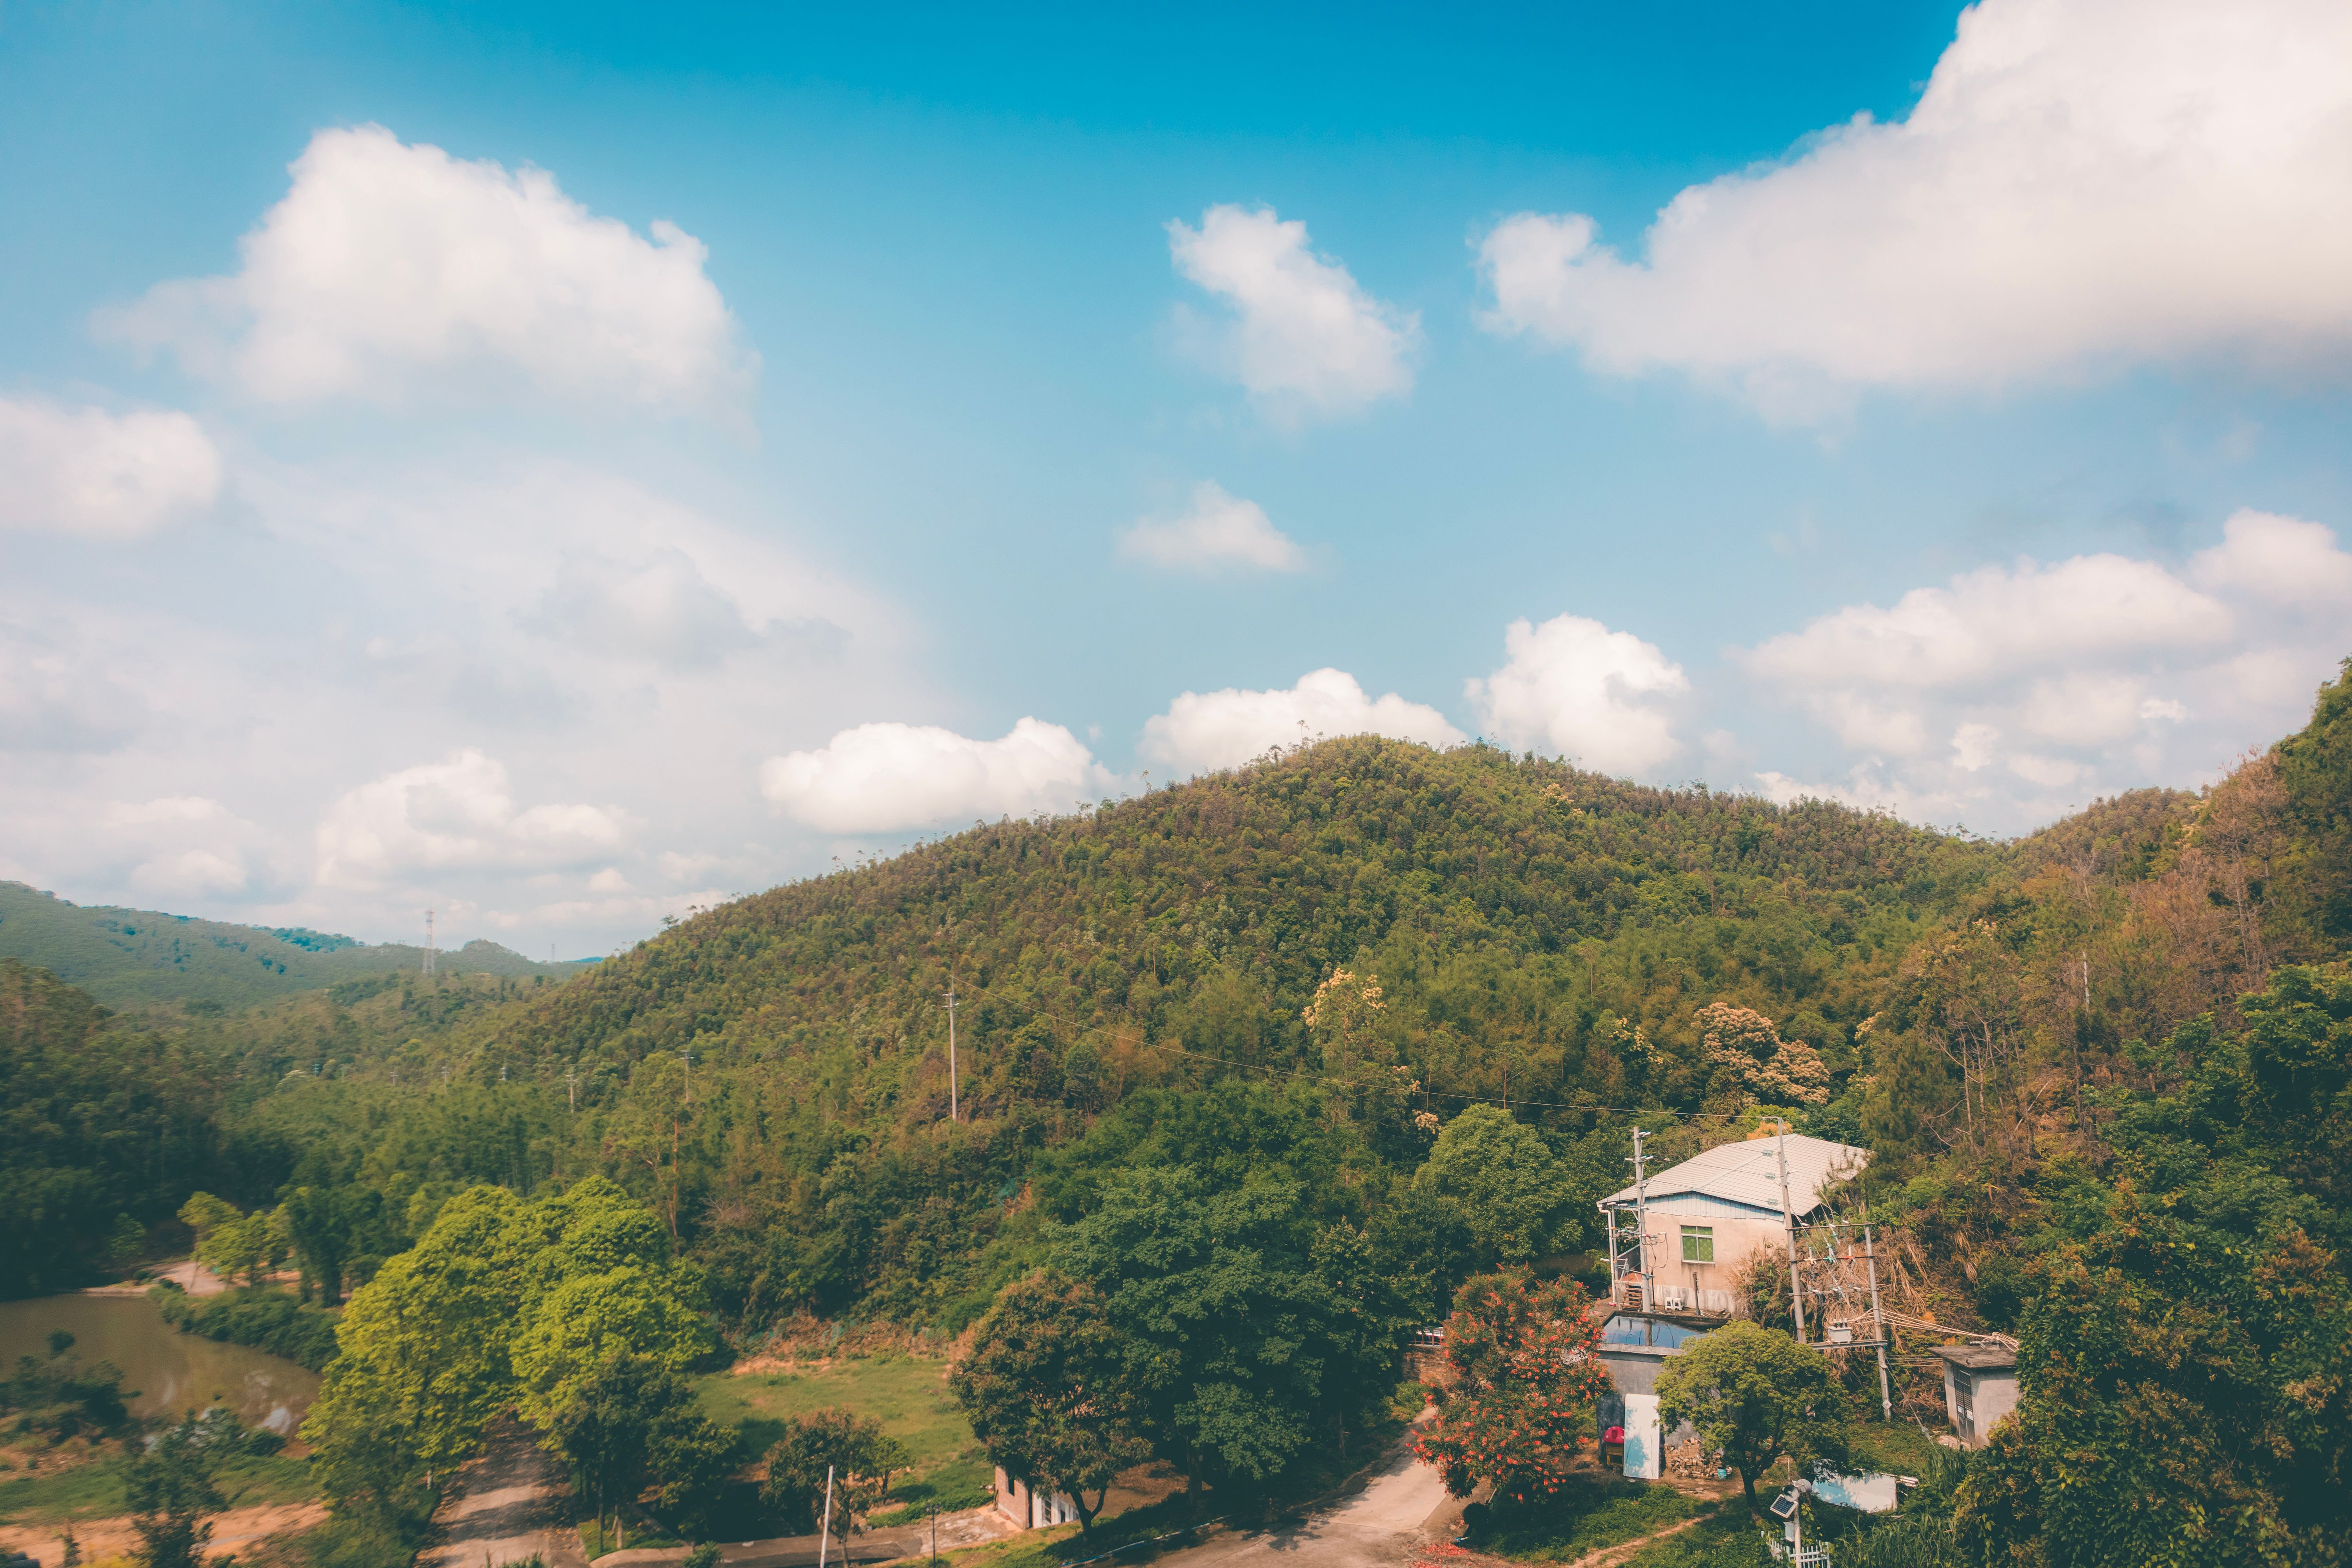
\includegraphics[width=0.7\textwidth]{./9280a1d42fa2.jpeg}
\end{center}
\end{frame}

\begin{frame}
\frametitle{图片解读：气候影响的缩影}
这张图片展示了气候变化引发的某一具体影响场景，例如冰川退缩、极端洪涝或生态系统退化的视觉证据。它与本节所述的多维影响遥相呼应——无论是海平面上升吞噬海岸线，还是极端天气摧毁家园，抑或是生态网络断裂，都提醒我们气候危机已不再是遥远的预测，而是正在发生的系统性风险。
\end{frame}

\begin{frame}
\frametitle{海平面上升：现状与未来风险}
\begin{itemize}
\item \alert{全球平均海平面}正以每年约\alert{3.7毫米}的速度上升，主要贡献来源几乎平分：冰川冰盖融化提供约50\%的水量，海水热膨胀贡献另外约50\%。自1993年卫星测高以来，全球海平面已累计升高约\alert{100毫米}。
\item 基于当前排放情景，到\alert{2050年}，全球沿海地区每年因海平面上升导致的直接经济损失可能突破\alert{1万亿美元}。包括上海、曼谷和迈阿密在内的超大城市将面临严峻的风暴潮与内涝风险，数以百万计的居民和关键基础设施暴露于危险之中。
\item 海平面上升还会通过盐水入侵破坏耕地和淡水资源，进一步加剧沿海生态系统的脆弱性，并可能引发资产贬值与保险市场动荡。
\end{itemize}
\end{frame}

\begin{frame}
\frametitle{生态系统承受重压：物种灭绝与海洋酸化}
\begin{itemize}
\item \textbf{物种灭绝风险}：联合国IPBES 2019年全球评估报告警告，约\alert{100万种物种}面临在未来数十年内灭绝的危险。\textbf{栖息地丧失}、\textbf{气候变化}和\textbf{污染}被列为三大驱动因素。气候变暖迫使物种迁移，破坏授粉、害虫控制等关键生态系统服务，直接威胁粮食安全与自然资本。
\item \textbf{海洋酸化}：海洋吸收了约\alert{30\%}的人为二氧化碳排放，导致海水表层pH值从工业化前的8.2降至\alert{8.1以下}（酸度增加约30\%）。酸化损害了珊瑚、贝类等钙化生物的造礁能力，\textbf{珊瑚白化事件}的频率自1980年代以来增加了\alert{5倍}，许多热带珊瑚礁已处于功能性崩溃的边缘。
\end{itemize}
\end{frame}

\begin{frame}
\frametitle{粮食安全的潜在危机：单产增速显著放缓}
\begin{itemize}
\item 全球主要粮食作物单产增速明显放缓：以小麦为例，全球平均单产年增长率从20世纪60年代的约\alert{3\%}下降至当前不足\alert{0.5\%}。\textbf{高温}和\textbf{水分胁迫}是核心制约因素。
\item 热浪导致作物在关键生长期（如灌浆期）遭受不可逆损害；降水模式的改变加剧了干旱和涝渍，限制了土壤水分供应；同时病虫害分布范围扩大，进一步削减产量。
\item 若升温趋势无法遏止，全球粮食系统的稳定性将面临前所未有的冲击，饥饿与营养不良人口可能显著反弹，尤其集中在非洲、南亚等气候脆弱区域。
\end{itemize}
\end{frame}

\begin{frame}
\frametitle{人类健康与极端事件的连锁冲击}
\begin{itemize}
\item \textbf{多重健康威胁}：气候变化通过\alert{热浪传染链}（直接中暑、心脑血管疾病）、\alert{媒介传播疾病范围扩大}（登革热、疟疾向高纬度和高海拔蔓延）以及\alert{粮食营养不良加剧}等途径，预估在\alert{2030年至2050年间}每年将增加约\alert{25万例额外死亡}。儿童、老年人和低收入群体承受着不成比例的脆弱性。
\item \textbf{极端事件案例：2022年巴基斯坦特大洪水}：该国遭受极端季风降雨叠加冰川融水，三分之一国土一度被淹没，超过\alert{3300万人}受灾，直接经济损失超过\alert{300亿美元}。这一事件被视为气候脆弱性国家的典型缩影，凸显了适应能力不足的国家面对气候冲击时的巨大代价。
\end{itemize}
\end{frame}

\begin{frame}
\frametitle{气候移民：2.16亿人的未来迁移}
\begin{itemize}
\item 世界银行2021年报告指出，到\alert{2050年}，气候变化可能迫使撒哈拉以南非洲、南亚和拉丁美洲约\alert{2.16亿人}在本国境内迁移。水资源短缺、农作物减产和海平面上升是主要推手。
\item 这种大规模内部迁移将给流入地区的城市承载能力、社会服务和就业市场带来严峻压力，可能激化资源竞争和社会紧张，形成连锁的政治安全挑战。
\item 气候移民已成为现实，而非未来的假设。制定前瞻性的适应与人口管理战略，已成为全球治理不可回避的议题。
\end{itemize}
\end{frame}

\section{全球应对策略：减缓、适应与技术路径}

\begin{frame}[fragile]\frametitle{本节导览}
\small
\begin{itemize}
    \item \textbf{全球气候治理}：《巴黎协定》与IPCC最新评估所设定的减排目标与路径
    \item \textbf{能源系统转型}：可再生能源成本骤降与创纪录的装机增长
    \item \textbf{碳移除与负排放}：CCUS技术进展和基于自然的解决方案
    \item \textbf{市场化政策工具}：碳定价机制的全球扩展与欧盟碳边界调整机制
    \item \textbf{气候适应实践}：以荷兰三角洲工程为代表的韧性基础设施典范
\end{itemize}
\end{frame}

\begin{frame}\frametitle{全球应对策略全景}
\begin{center}
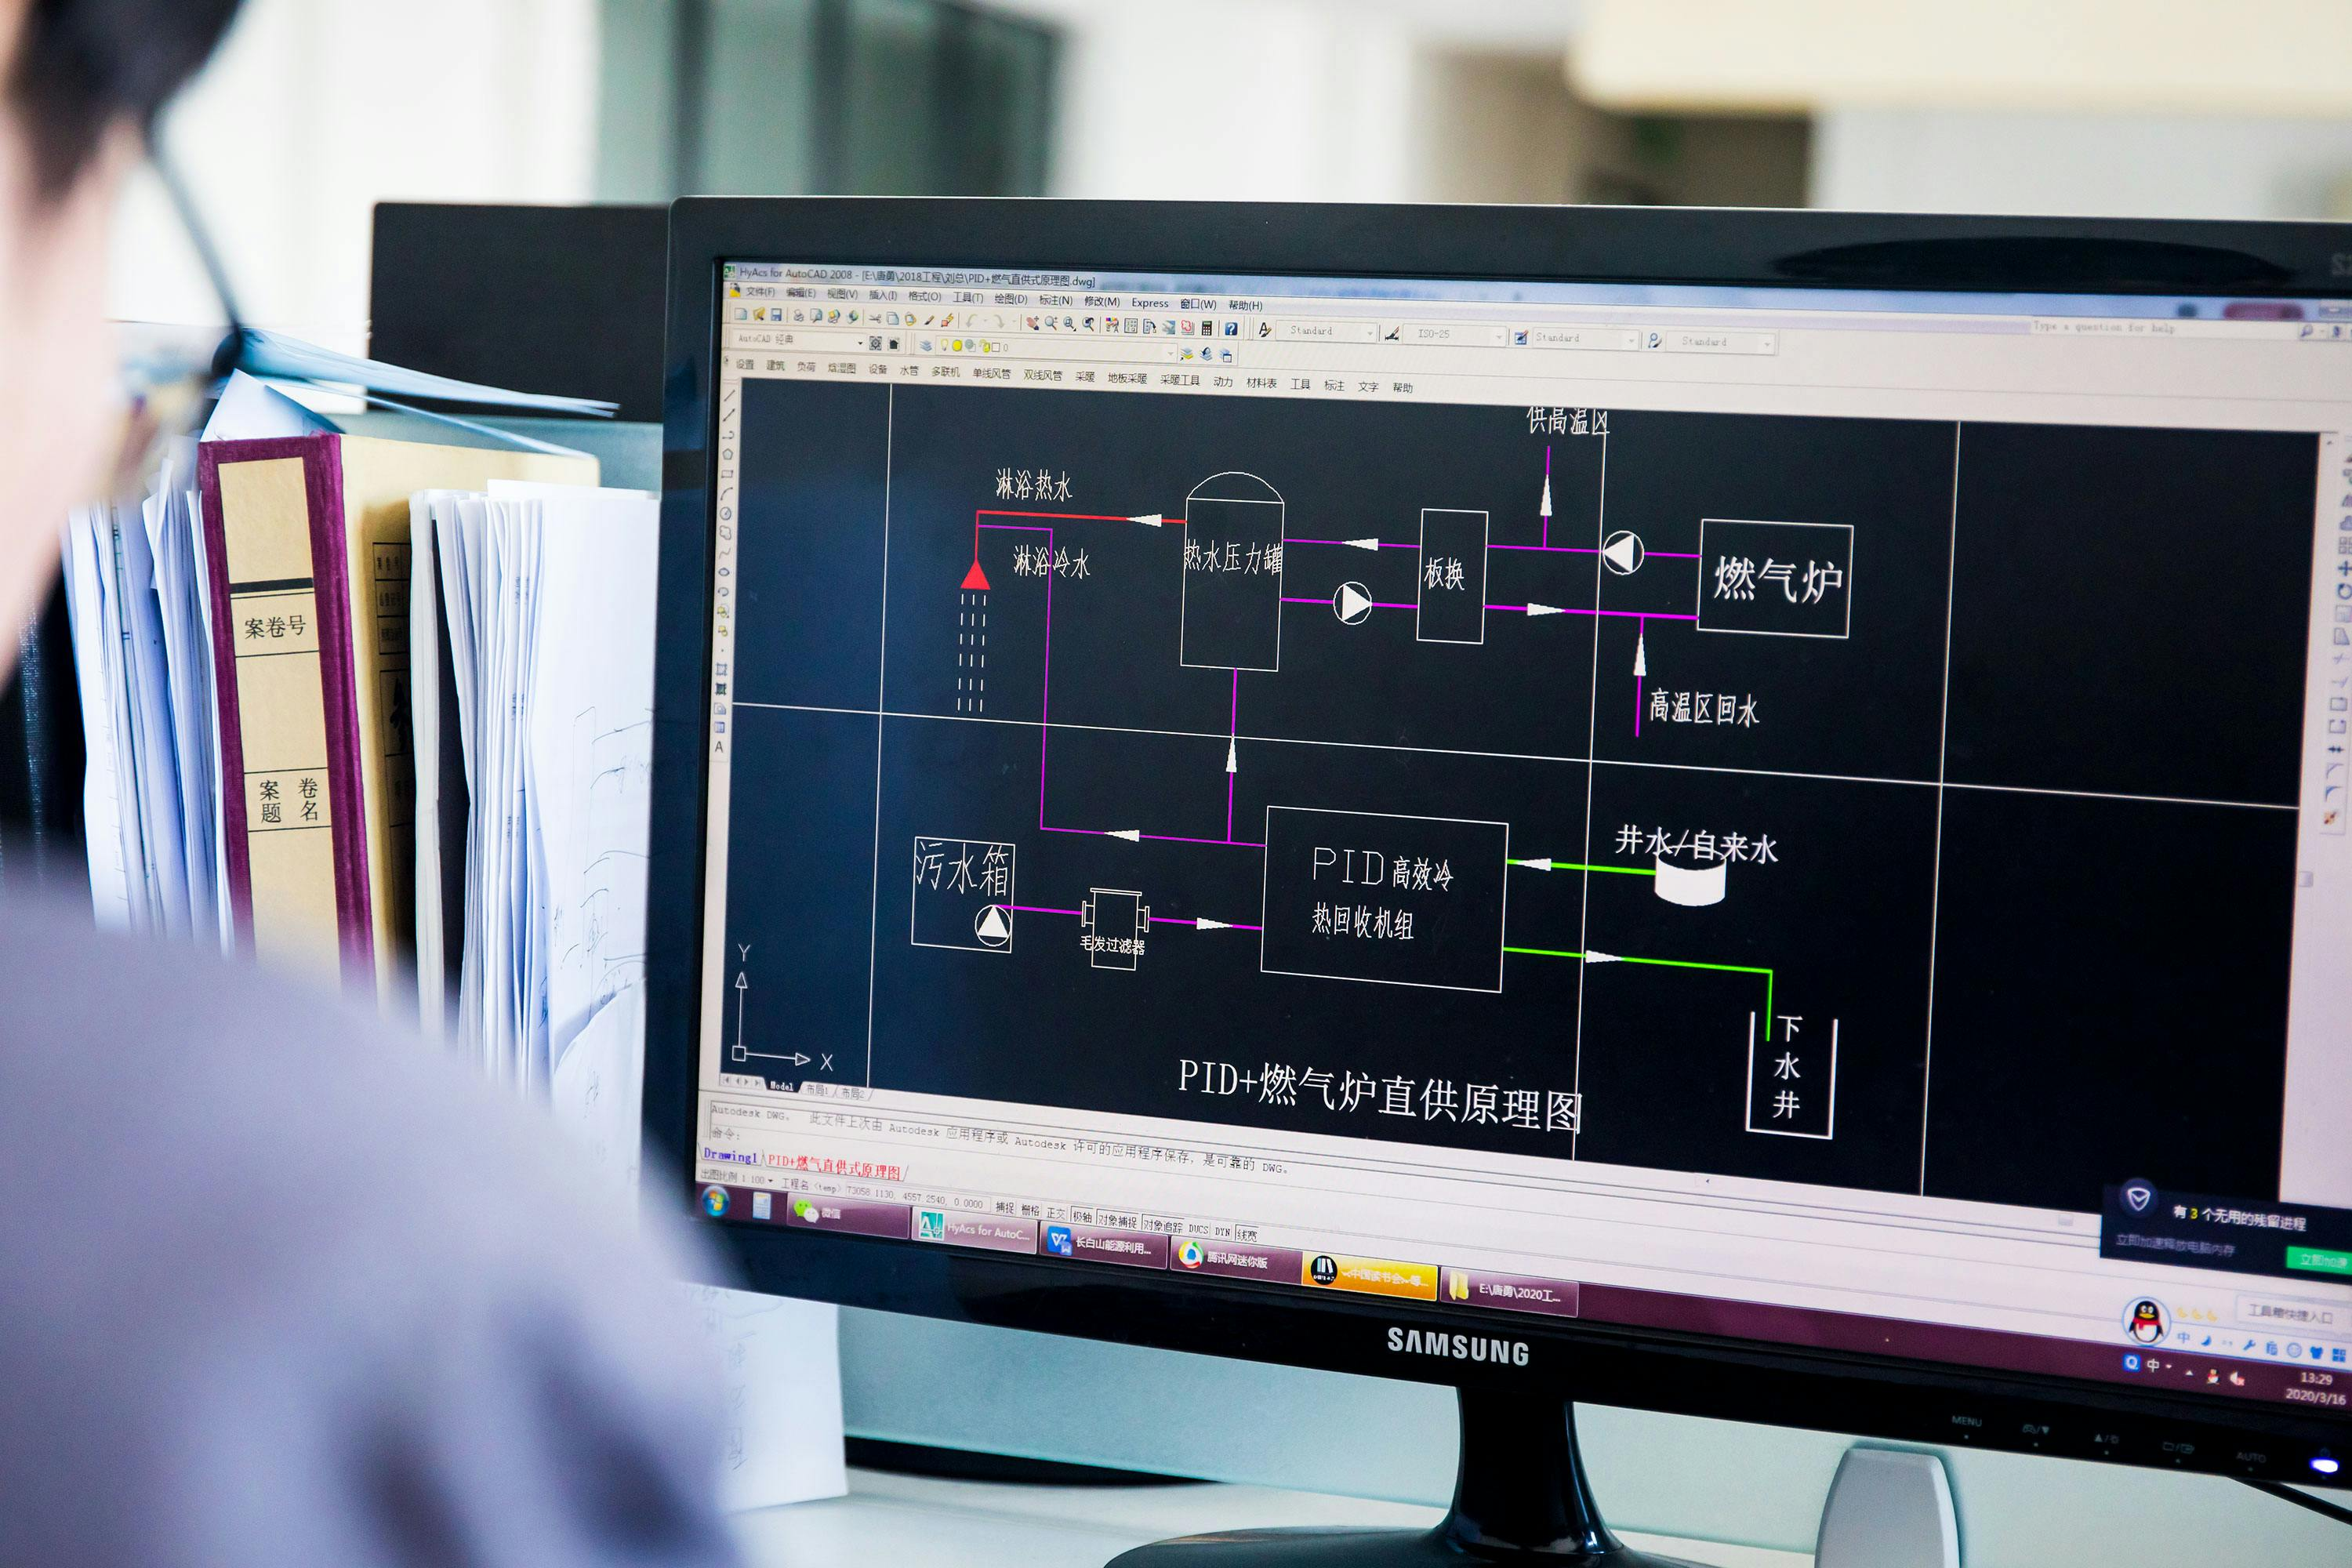
\includegraphics[width=0.7\textwidth]{./2ba8a2418030.jpeg}
\end{center}
\end{frame}

\begin{frame}\frametitle{图片解读：系统化的应对路径}
\small
该图将减缓、适应、技术革新与政策工具等多个维度的应对策略有机串联起来。它直观地展示了从能源转型、自然解决方案到碳定价和气候韧性建设的协同关系，与本节将要深入讨论的全球应对框架高度呼应，突显了实现《巴黎协定》目标所需的多元联动路径。
\end{frame}

\begin{frame}\frametitle{国际气候治理与减排路径}
\small
\begin{itemize}
    \item \textbf{《巴黎协定》与全球自主贡献}\\
    《巴黎协定》于2015年底达成，2016年快速生效，明确将全球平均气温升幅控制在工业化前水平以上\alert{2℃以内}，并努力限制在\alert{1.5℃}。截至目前，已有194个缔约方提交了国家自主贡献方案，覆盖超过全球排放量的95\%。协定还建立了全球盘点机制，每五年评估集体进展，推动各国逐步提升雄心。
    
    \item \textbf{IPCC第六次评估报告的紧迫时间表}\\
    政府间气候变化专门委员会第六次评估报告明确指出，要实现1.5℃目标，全球温室气体排放需在\alert{2025年前}达到峰值，并在2030年相比2019年水平\alert{减少约43\%}。这意味着未来几年是决定性的窗口期，任何延迟都将急剧增加超过临界点的风险，并大幅抬高转型成本。
\end{itemize}
\end{frame}

\begin{frame}\frametitle{能源转型：成本革命与加速部署}
\small
\begin{itemize}
    \item \textbf{太阳能光伏成本的历史性下降}\\
    全球太阳能光伏加权平均平准化度电成本从2010年的约\alert{0.381美元/千瓦时}骤降至2022年的\alert{0.049美元/千瓦时}，降幅接近85\%。这使得太阳能光伏在越来越多的地区成为最廉价的新建电源，彻底改变了电力经济格局，为中国、印度等国的煤电替代提供了强大经济驱动力。
    
    \item \textbf{2022年可再生能源新增装机的里程碑}\\
    2022年全球可再生能源新增装机容量达到创纪录的约\alert{295吉瓦}，其中太阳能光伏和风电合计占比超过90\%。这一数字标志着全球能源转型已进入关键加速期，投资重心正从化石能源向清洁电力不可逆转地转移，且新兴市场和发展中国家的贡献日益显著。
\end{itemize}
\end{frame}

\begin{frame}\frametitle{碳捕获、利用与封存（CCUS）}
\small
\begin{itemize}
    \item \textbf{针对难以脱碳行业的补充路径}\\
    CCUS被定位为水泥、钢铁、化工等难以通过电气化脱碳行业的\alert{补充手段}，是实现净零排放不可或缺的技术组合之一。截至2023年，全球在运CCUS设施的总捕获能力约为\alert{4400万吨二氧化碳/年}，大部分集中于天然气加工和提高石油采收率项目。
    
    \item \textbf{大规模商业化部署的前景}\\
    国际能源署等机构预测，2030年后CCUS将迎来大规模商业化部署，多个百万吨级项目已在北美、欧洲和亚太地区规划或建设。但当前仍面临成本偏高、封存场地选择和社会接受度等挑战，需要政策激励、集群化基础设施和碳差价合约等创新工具来加速规模化。
\end{itemize}
\end{frame}

\begin{frame}\frametitle{基于自然的解决方案（NbS）}
\small
\begin{itemize}
    \item \textbf{低成本且高协同效益的减排途径}\\
    基于自然的解决方案包括大规模造林再造林、湿地恢复、红树林保护和碳汇农业等，据估算这些措施到2030年能以\alert{较低成本}贡献全球所需减排量的约\alert{30\%}。它们不仅固碳，还能提升生物多样性、改善水质、保障粮食安全，体现出气候变化与生态保护的协同效应。
    
    \item \textbf{典型案例与潜在规模}\\
    中国的塞罕坝人工林、非洲“绿色长城”等大规模生态工程已展现出NbS的实际效果。IPCC特别报告强调，通过修复退化的森林和土壤，每年可封存数十亿吨二氧化碳，同时增强社区对极端气候的适应能力，使NbS成为最具成本效益的综合应对手段之一。
\end{itemize}
\end{frame}

\begin{frame}\frametitle{碳定价机制与国际协调}
\small
\begin{itemize}
    \item \textbf{碳定价工具的全球扩展}\\
    截至2023年，全球共有\alert{73个}碳定价工具投入运行，涵盖碳税和排放交易体系，覆盖约\alert{23\%}的全球温室气体排放。欧盟、中国、韩国等主要经济体均已建立碳排放交易市场，2021年中国全国碳市场启动，覆盖电力行业超过40亿吨二氧化碳，成为全球覆盖排放量最大的碳市场。
    
    \item \textbf{欧盟碳边界调整机制与碳成本趋同}\\
    欧盟碳边界调整机制（CBAM）于\alert{2023年10月}进入过渡期，要求进口商报告水泥、钢铁、电力等产品的隐含碳排放，并将在2026年正式征收碳差价。这一机制旨在防止碳泄漏，推动国际贸易伙伴加快碳定价，逐步形成全球碳成本趋同的态势，引发全球供应链的深层调整。
\end{itemize}
\end{frame}

\begin{frame}\frametitle{适应策略：荷兰三角洲工程}
\small
\begin{itemize}
    \item \textbf{气候适应性水利工程的全球典范}\\
    荷兰“三角洲工程”是世界上规模最大、技术最先进的防潮工程之一，通过\alert{可升降闸门}、\alert{风暴潮屏障}和强化堤防构建起多层次防御体系。它直接响应1953年北海大洪水的惨痛教训，使荷兰这一低地国家能够抵御万年一遇的极端海况，成为全球气候适应性基础设施设计的参照样板。
    
    \item \textbf{成功实践与推广价值}\\
    该工程已成功抵御多次极端海况事件，包括1990年代和2010年代的强烈风暴潮，避免了大规模人员伤亡和经济损失。其核心理念——将硬性工程与基于自然的柔性防护（如沙滩补砂）相结合，已被越南、美国、孟加拉国等面临海平面上升威胁的国家借鉴和本土化应用。
\end{itemize}
\end{frame}

\section{案例与实践：国家、城市与行业层面的绿色转型}

\begin{frame}\frametitle{本节概览：绿色转型的多维实践}
\begin{itemize}
    \item \textbf{国家路径}：哥斯达黎加与德国的可再生能源革命
    \item \textbf{大国承诺}：中国的碳达峰碳中和行动与能源转型
    \item \textbf{城市先锋}：哥本哈根与C40联盟的碳中和目标
    \item \textbf{企业重塑}：沃旭能源与特斯拉的绿色产业引领
    \item \textbf{科技赋能}：全球森林观察平台的卫星监测实践
\end{itemize}
\end{frame}

\begin{frame}\frametitle{全球绿色转型图景}
\begin{center}
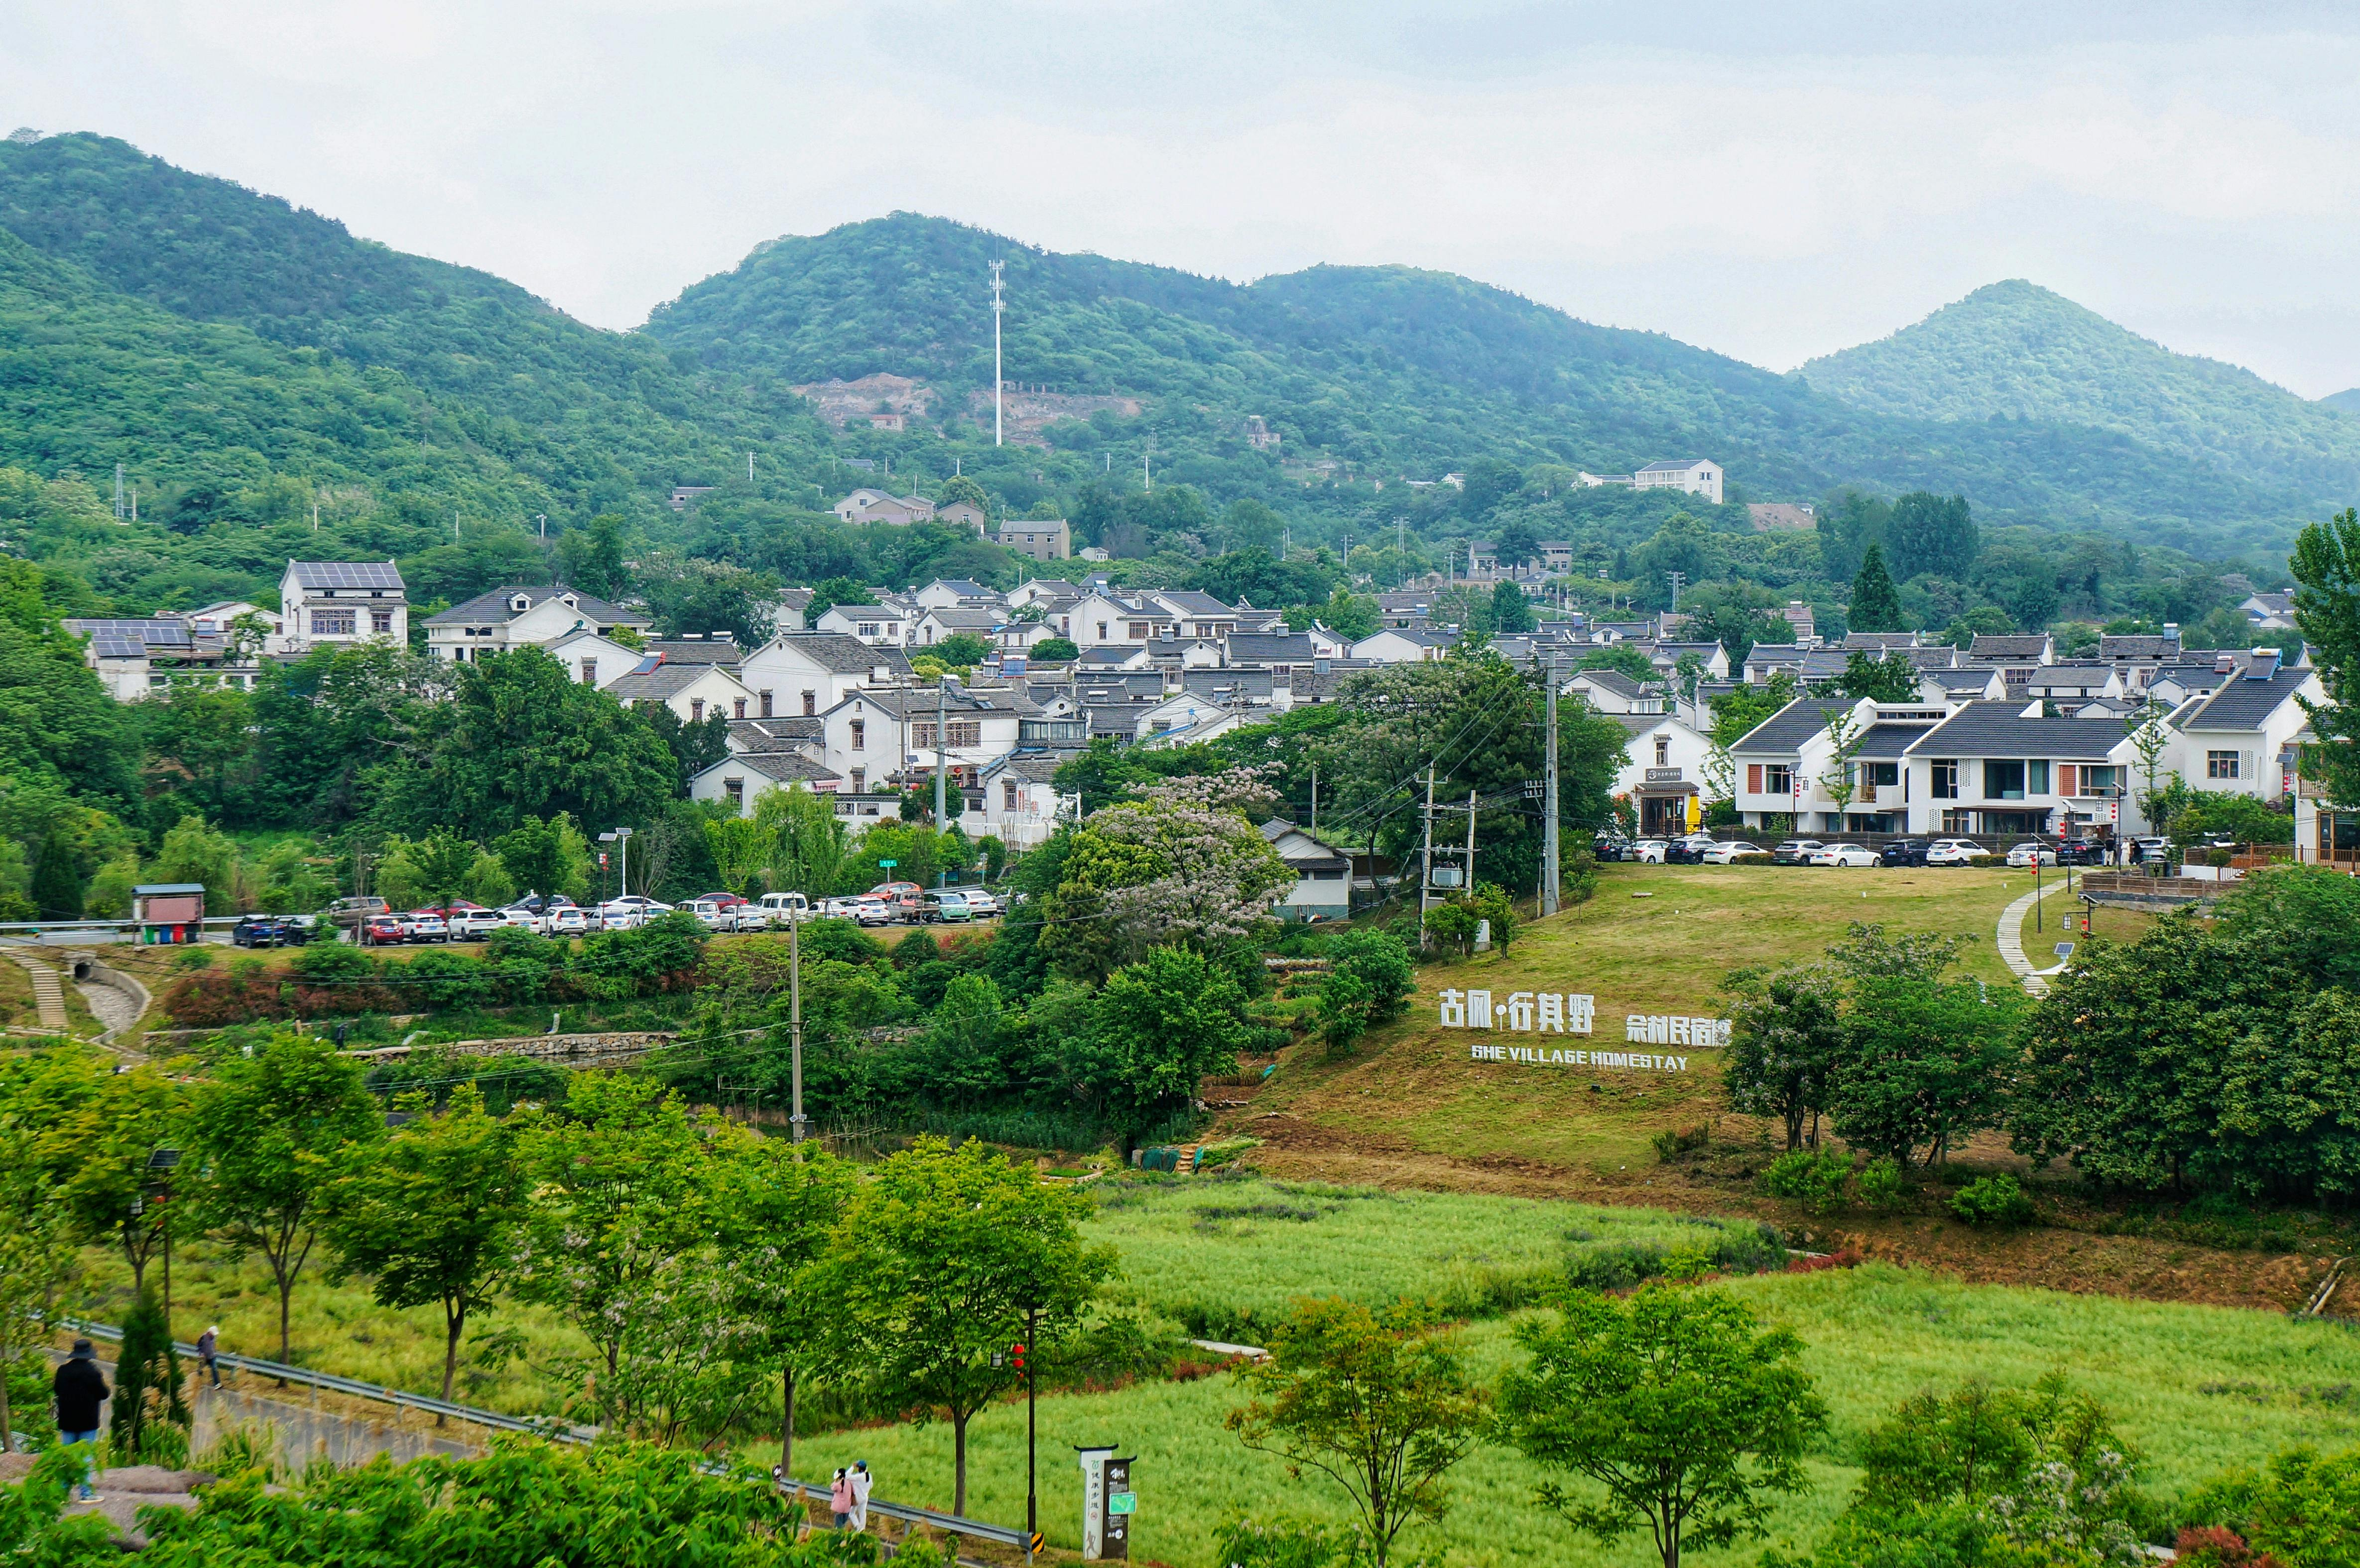
\includegraphics[width=0.7\textwidth]{./9dd26189f1f8.jpeg}
\end{center}
\end{frame}

\begin{frame}\frametitle{图片解读：多元力量共筑绿色未来}
本节从国家政策、城市规划和行业创新等维度，剖析全球绿色转型的典型案例。配图呼应了这一多层级、多主体协同推进的格局——从清洁能源基础设施到可持续城市设计，再到基于科技的生态守护，共同勾勒出一幅由承诺走向行动的全球图景。
\end{frame}

\begin{frame}\frametitle{国家绿色转型案例（一）：哥斯达黎加与德国}
\begin{itemize}
    \item \textbf{哥斯达黎加：从清洁电力到“碳中和国家”品牌}
    \begin{itemize}
        \item 自2015年以来，该国已连续8年实现全国超过98\%的电力来自可再生能源，主要依托丰富的水电、地热和风能资源。
        \item 政府将这一成就成功转化为“碳中和国家”品牌，极大地拉动了生态旅游业，目前该行业约占GDP的8\%，成为小国可持续发展的全球范本。
    \end{itemize}
    \vspace{0.3cm}
    \item \textbf{德国：\alert{《可再生能源法》}与能源民主化}
    \begin{itemize}
        \item 2000年实施的《可再生能源法》奠定了固定上网电价机制，推动2022年可再生能源发电占比达到46\%，并明确2030年80\%的目标。
        \item 通过补贴和竞价体系，德国培育出大量分散式\textbf{公民能源合作社}，让普通民众直接参与能源转型，实现了经济效益与公众赋权的双赢。
    \end{itemize}
\end{itemize}
\end{frame}

\begin{frame}\frametitle{国家绿色转型案例（二）：中国的双碳行动}
\begin{itemize}
    \item \textbf{全球最大碳排放国的雄心}
    \begin{itemize}
        \item 2020年，中国正式提出2030年前实现\textbf{碳达峰}、2060年前实现\textbf{碳中和}的目标，为全球气候治理注入关键动能。
        \item 截至2023年底，全国风电和光伏装机总量已突破1000吉瓦，占全球三分之一以上，非化石能源占比稳步提升。
    \end{itemize}
    \vspace{0.2cm}
    \item \textbf{碳市场与系统转型}
    \begin{itemize}
        \item 中国建成了全球覆盖人口最多的\textbf{碳排放权交易市场}，率先纳入电力行业，并在逐步扩大至钢铁、水泥等高排放部门。
        \item 结合大规模风光基地、特高压输电和储能建设，中国正在从“煤基巨人”向绿色低碳体系快速转身。
    \end{itemize}
\end{itemize}
\end{frame}

\begin{frame}\frametitle{城市绿色转型：哥本哈根与C40联盟}
\begin{itemize}
    \item \textbf{哥本哈根：迈向首个碳中和首都}
    \begin{itemize}
        \item 该市制定了2025年成为全球首个碳中和首都的目标，依靠\textbf{区域供热系统}覆盖绝大部分建筑，并大力推行建筑节能改造。
        \item 通过长达数百公里的独立自行车道网络，市内出行中\textbf{自行车占比高达62\%}，配合绿色交通政策，2005年以来碳排放已下降约70\%。
    \end{itemize}
    \vspace{0.2cm}
    \item \textbf{C40城市气候领导联盟：集体行动的力量}
    \begin{itemize}
        \item 全球已有超过100个城市加入C40，成员合计实施了超过12\,000项气候行动，从建筑能效到零碳交通全面铺开。
        \item \alert{洛杉矶的“绿色新政”}规划到2035年实现100\%可再生能源供电，并预计创造约40万个绿色就业岗位，展示了城市层级引领公正转型的潜力。
    \end{itemize}
\end{itemize}
\end{frame}

\begin{frame}\frametitle{企业绿色转型：沃旭能源与特斯拉}
\begin{itemize}
    \item \textbf{沃旭能源：从油气巨头到海上风电领跑者}
    \begin{itemize}
        \item 这家丹麦能源企业十年内剥离了所有化石燃料资产，转型为全球最大的\textbf{海上风电}开发商。
        \item 2021年，其海上风电场贡献了全球约三分之一的安装容量，证明了传统能源公司彻底脱碳的商业可行性。
    \end{itemize}
    \vspace{0.2cm}
    \item \textbf{特斯拉：加速道路交通电气化}
    \begin{itemize}
        \item 通过电动汽车和家用储能系统的规模化生产，特斯拉2023年全球交付量超过180万辆，成为行业变革的催化剂。
        \item 在其推动下，全球乘用电动车销量占比从2019年的2.5\%快速上升至2023年的约15\%，显著挤压燃油车市场空间。
    \end{itemize}
\end{itemize}
\end{frame}

\begin{frame}\frametitle{科技监测：全球森林观察与卫星透明化}
\begin{itemize}
    \item \textbf{近实时的森林碳损失监测}
    \begin{itemize}
        \item “全球森林观察”平台融合Landsat和哨兵系列卫星数据，实现了对全球热带雨林\textbf{近实时}的碳损失追踪与可视化。
        \item 该平台为亚马逊流域各国的执法部门和NGO提供了客观、透明化的毁林数据，极大压缩了非法砍伐的信息盲区。
    \end{itemize}
    \vspace{0.2cm}
    \item \textbf{数据驱动保护}
    \begin{itemize}
        \item 透明的遥感监测已促成部分地区森林砍伐率的显著下降，成为科技赋能气候行动和生物多样性保护的标杆案例。
        \item 这种将大规模卫星数据转化为决策工具的模式，正在被复制到其他生态系统的保护中。
    \end{itemize}
\end{itemize}
\end{frame}

\section{个人行动与未来展望：从碳足迹到系统性变革}

\begin{frame}
\frametitle{本节概览：从个体选择到文明重塑}
本讲聚焦个体责任与系统变革的双重路径，核心议题包括：
\begin{itemize}
    \item \textbf{居民消费碳足迹：}全球排放的真正源头，四大板块的核算与悬殊差异
    \item \textbf{衣食住行的绿色转型：}出行与饮食的减排潜力、家庭节能的实践回报
    \item \textbf{青年运动与技术突破：}社会动员与下一代脱碳技术的前沿动态
    \item \textbf{系统性深度变革：}补贴改革、财务披露与超越GDP的新文明指标
    \item \textbf{从风险到契机：}碳中和文明如何在行星边界内实现再生与繁荣
\end{itemize}
\end{frame}

\begin{frame}
\frametitle{配图：变革力量的交汇}
\begin{center}
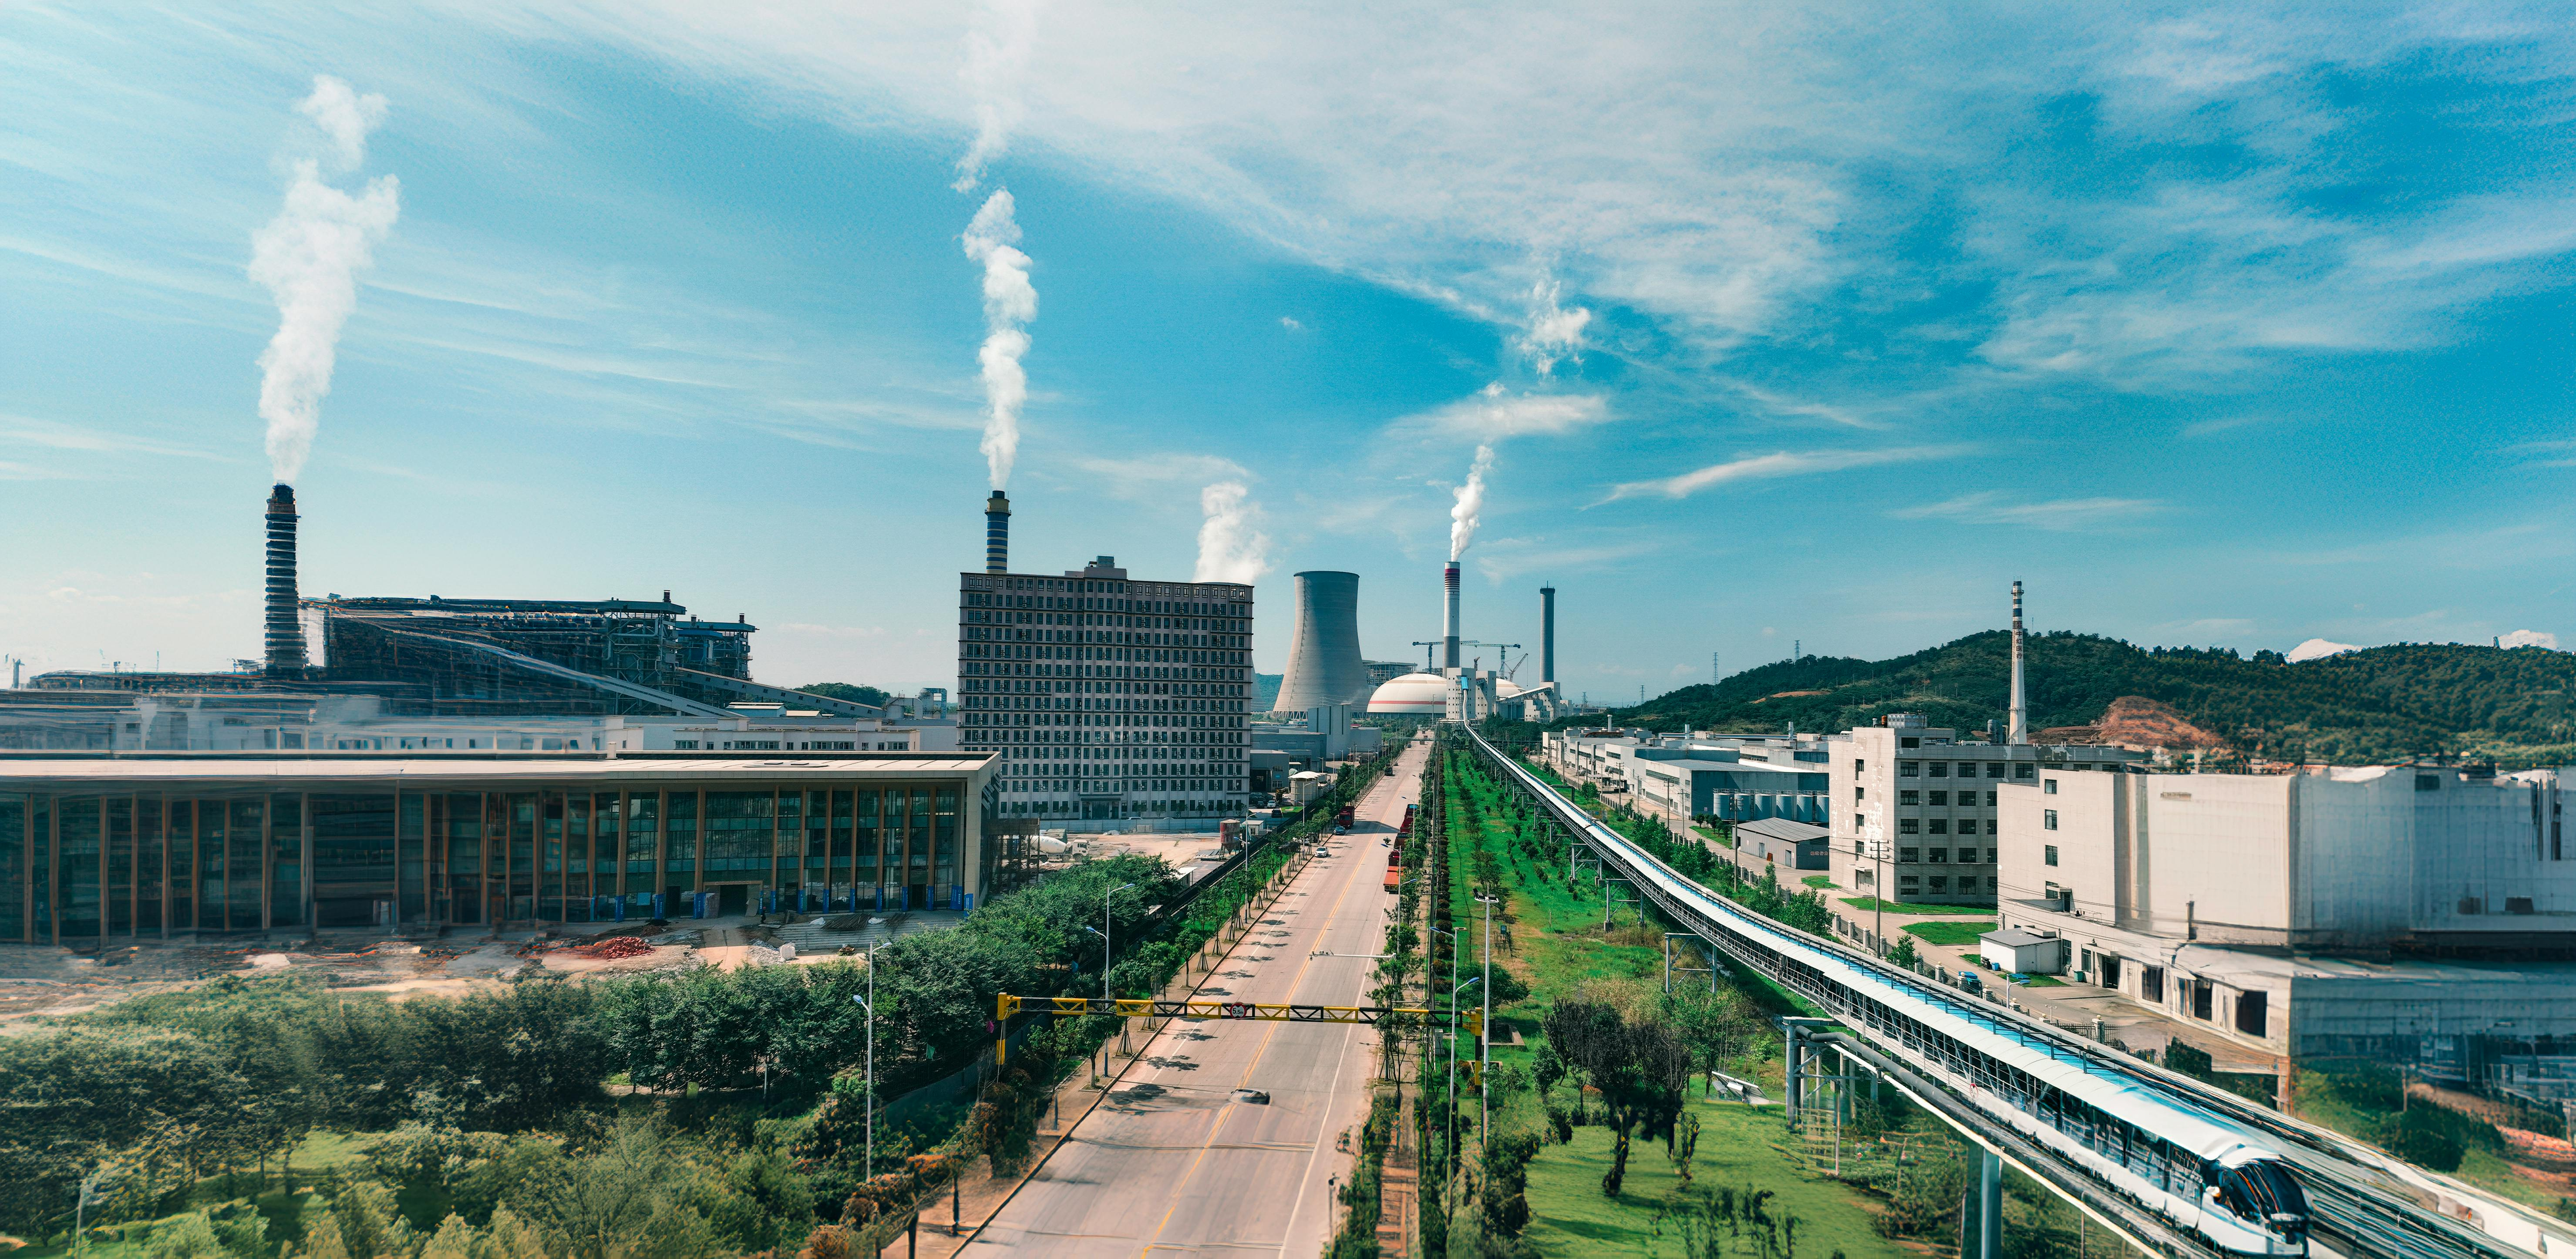
\includegraphics[width=0.7\textwidth]{./f466b5bcc76b.jpeg}
\end{center}
\end{frame}

\begin{frame}
\frametitle{图片解读：个体行动与系统愿景的结合}
这幅画面浓缩了本节的核心张力——\textbf{微小的日常选择与宏大的系统转型并非对立，而是同一场变革的两面}。图中可能呈现的城市农场、自行车道、屋顶光伏或气候罢工的视觉元素，恰恰呼应了我们即将讨论的饮食结构调整、绿色出行、家庭节能和青年动员。它提醒我们，\alert{每一个碳足迹的缩减都与政策窗口的打开、技术成本的下降以及文化叙事的变化紧密相连}，这也是我们理解“从碳足迹到系统性变革”这一主题的关键视角。
\end{frame}

\begin{frame}
\frametitle{被忽视的源头：居民消费碳足迹}
\begin{itemize}
    \item 全球温室气体排放的 \textbf{60\%--70\%} 最终由居民消费驱动，意味着“谁消费、谁负责”的原则正成为气候治理的新基线。碳足迹核算通常覆盖 \alert{住房（供暖、制冷、电力）}、\alert{交通（私家车、航空）}、\alert{食品（肉类、乳制品）}和\alert{消费品（服装、电子产品）}四大板块。
    \item 人均排放的鸿沟极为惊人：\textbf{北美和部分欧洲高收入国家}人均年碳排放可达15--20吨，而\alert{撒哈拉以南非洲多数国家仍不足1吨}。这一差距不仅反映生活方式，更指向历史责任与气候正义的深层矛盾。
    \item 理解碳足迹并非为了制造道德负担，而是提供精准干预的依据——例如，一项针对英国消费者的研究发现，\textbf{在不显著降低生活质量的前提下，仅通过优化饮食、出行和能效，即可削减30\%--50\%的个人碳足迹}。
\end{itemize}
\end{frame}

\begin{frame}
\frametitle{移动与饮食：高回报的个人减排杠杆}
\framesubtitle{绿色出行与饮食结构转型}
\begin{itemize}
    \item \textbf{出行领域：}将每周一次的中长途汽车出行转为高铁，可\alert{减少约90\%的碳排放}；而纯电动汽车在全生命周期内的碳排放仅为传统燃油车的一半，且将随着电网中可再生能源比例的提高而进一步下降。在挪威，纯电动车市场份额已超过80\%，证明政策激励与基础设施布局可以有效改变私人交通结构。
    \item \textbf{饮食转向：}采用以植物基为主的弹性饮食（flexitarian diet）可将\alert{全球食品相关温室气体排放在2050年前削减多达60\%}。这并非要求全民成为严格素食者，而是将红肉和奶制品消费降低至健康与行星边界都能接受的水平。
    \item 饮食转型还带来巨大的\alert{协同效益}——释放出数百万平方公里的农业用地，这些土地通过重新造林或湿地恢复可以转变为活跃的碳汇，同时保护濒危生物多样性热点。EAT-《柳叶刀》委员会的研究为此提供了可量化的科学框架。
\end{itemize}
\end{frame}

\begin{frame}
\frametitle{家庭节能：看得见的减排与节省}
\begin{itemize}
    \item 建筑运行占全球碳排放的近30\%，而家庭层面的改造具有\alert{投资小、回报快}的特点。选择\alert{最高能效等级的电器}、增加阁楼与墙体隔热、全面换装LED照明并安装智能温控器，这些措施的叠加效果远超单点行动。
    \item 美国“能源之星”（ENERGY STAR）计划的数据显示，参与该计划的家庭平均可削减\alert{20\%的能源消费}，而增量改造成本通常\alert{5年内即可通过节约的电费与燃气费完全收回}。类似地，欧盟的能效标签制度也推动了每年数百亿欧元的消费者节约。
    \item 值得注意的是，\textbf{行为层面的调整}——如冬季供暖温度降低1°C、缩短淋浴时间、合理利用自然通风——几乎零成本，却可以对家庭碳足迹产生5\%--10\%的削减，这些“隐性杠杆”在气候传播中应被更多强调。
\end{itemize}
\end{frame}

\begin{frame}
\frametitle{公民力量与下一代技术窗口}
\framesubtitle{青年运动与前沿脱碳技术}
\begin{itemize}
    \item \textbf{青年主导的气候运动}自2018年秋季“未来星期五”（Fridays for Future）爆发以来，彻底改写了全球政策议程。瑞典青年格蕾塔·桑伯格发起的校园罢工迅速席卷\alert{超过150个国家}，数百万学生走上街头，催生了英国、加拿大、法国等多国议会宣布\alert{“气候紧急状态”}，直接推动了更陡峭的减排目标立法。
    \item 这一代青年将气候变化重新定义为\alert{生存危机与道德急务}，其影响力不仅停留于街头，更渗透进法庭（气候诉讼）和董事会（迫使金融机构重新评估化石能源投资），证明了公民社会在加速转型中不可替代的作用。
    \item \textbf{技术前沿}正为深度脱碳补齐缺口：\alert{长时储能}（如铁-空气电池、重力储能）解决可再生能源的间歇性；\alert{绿色氢能}通过电解水制氢，国际能源署预计其成本到2030年有望降至2美元/公斤以下，使钢铁、化工、航运等“难减排行业”看到可行出路；\alert{直接空气捕获（DAC）}则进入示范阶段，虽成本仍高，但其作为“碳移除负排放技术”的角色已不可忽视。
\end{itemize}
\end{frame}

\begin{frame}
\frametitle{系统性变革的三重引擎与文明升华}
\framesubtitle{政策、金融与文化协同转型}
\begin{itemize}
    \item \textbf{政策转向：}国际货币基金组织指出，2022年全球化石燃料的显性与隐性补贴合计高达\alert{惊人的7万亿美元}，相当于全球GDP的7.1\%，取消化石燃料补贴并实行碳定价，是释放市场转向清洁能源的最有效手段。同时，强制性\alert{气候相关财务信息披露（如TCFD、ISSB标准）}正使气候风险成为董事会决策的核心变量。
    \item \textbf{文化指标的重塑：}越来越多的思想者呼吁超越GDP，建立以“可持续福祉”为核心的新指标体系（如\alert{真实发展指标GPI、甜甜圈经济模型}），甚至严肃探讨“去增长”（degrowth）在北半球高收入国家的适用性。不丹的国民幸福总值（GNH）实践、苏格兰的福祉经济框架都是可借鉴的范例。
    \item \textbf{终极视角：}气候变化叙事完全可以从“危局”升华为\alert{文明升级的契机}。将\alert{地球系统边界（行星边界九维度）}作为社会经济发展的刚性约束，人类有望在21世纪中叶构建一种\alert{气候韧性、碳中和且生态再生的新文明形态}——这不仅是风险应对，更是人类集体智慧与协作的巅峰展现。
\end{itemize}
\end{frame}

\end{document}